\section{多变量函数的 Taylor 公式与极值}

\begin{problem}{全微分与复合函数求导}{Chain-Rule-Slope}
    求曲线 $F(t) = f(x + th, y + tk)$ 在 $t = 1$ 处的斜率, 其中
    \begin{enumerate}
        \item $f(x, y) = \sin(x^{2} + y)$;
        \item $f(x, y) = x^{2} + 2xy^{2} - y^{4}$.
    \end{enumerate}
\end{problem}

\begin{solution}
    由复合函数求导法则, $F(t)$ 关于 $t$ 的导数为
    \begin{equation}
        F'(t) = f_{x}(x+th, y+tk) \cdot h + f_{y}(x+th, y+tk) \cdot k
    \end{equation}

    \ansitem{1}

    计算偏导数得
    \begin{equation}
        f_{x} = 2x \cos(x^2 + y), \quad f_{y} = \cos(x^2 + y)
    \end{equation}
    将其代入 $F'(1)$ 的表达式中
    \begin{equation}
        \begin{aligned}
            F'(1) & = 2(x+h) \cos((x+h)^2 + (y+k)) \cdot h + \cos((x+h)^2 + (y+k)) \cdot k \\
                  & = [2(x+h)h + k] \cos((x+h)^2 + (y+k))
        \end{aligned}
    \end{equation}
    \begin{equation}
        \boxed{F'(1) = [2(x+h)h + k] \cos((x+h)^2 + (y+k))}
    \end{equation}

    \ansitem{2}

    计算偏导数得
    \begin{equation}
        f_{x} = 2x + 2y^2, \quad f_{y} = 4xy - 4y^3
    \end{equation}
    将其代入 $F'(1)$ 的表达式中
    \begin{equation}
        \begin{aligned}
            F'(1) & = [2(x+h) + 2(y+k)^2]h + [4(x+h)(y+k) - 4(y+k)^3]k \\
                  & = 2h(x + h + (y+k)^2) + 4k(y+k)(x + h - (y+k)^2)
        \end{aligned}
    \end{equation}
    \begin{equation}
        \boxed{F'(1) = 2h(x + h + (y+k)^2) + 4k(y+k)(x + h - (y+k)^2)}
    \end{equation}
\end{solution}


\begin{problem}{多元函数增量}{Function-Increment}
    求下列函数由点 $(x_{0}, y_{0})$ 变到 $(x_{0} + h, y_{0} + k)$ 时函数的增量.
    \begin{enumerate}
        \item $f(x, y) = x^{3} + y^{2} - 6xy - 39x + 18y + 4$, $(x_{0}, y_{0}) = (5, 6)$;
        \item $f(x, y) = x^{2}y + xy^{2} - 2xy$, $(x_{0}, y_{0}) = (1, -1)$.
    \end{enumerate}
\end{problem}

\begin{solution}
    利用泰勒展开式计算增量 $\Delta f = f(x_0+h, y_0+k) - f(x_0, y_0)$.

    \ansitem{1}

    计算点 $(5, 6)$ 处的各阶偏导数
    \begin{equation}
        \begin{aligned}
            f_{x}   & = 3x^2 - 6y - 39 \implies f_x(5, 6) = 0                              \\
            f_{y}   & = 2y - 6x + 18 \implies f_y(5, 6) = 0                                \\
            f_{xx}  & = 6x \implies f_{xx}(5, 6) = 30, \quad f_{xy} = -6, \quad f_{yy} = 2 \\
            f_{xxx} & = 6, \quad \text{其余高阶偏导数均为 } 0
        \end{aligned}
    \end{equation}
    代入泰勒公式
    \begin{equation}
        \begin{aligned}
            \Delta f & = \frac{1}{2}(30h^2 - 12hk + 2k^2) + \frac{1}{6}(6h^3) \\
                     & = 15h^2 - 6hk + k^2 + h^3
        \end{aligned}
    \end{equation}
    \begin{equation}
        \boxed{\Delta f = 15h^2 - 6hk + k^2 + h^3}
    \end{equation}

    \ansitem{2}

    计算点 $(1, -1)$ 处的各阶偏导数
    \begin{equation}
        \begin{aligned}
            f_{x}   & = 2xy + y^2 - 2y \implies f_x(1, -1) = 1                                           \\
            f_{y}   & = x^2 + 2xy - 2x \implies f_y(1, -1) = -3                                          \\
            f_{xx}  & = 2y \implies -2, \quad f_{xy} = 2x+2y-2 \implies -2, \quad f_{yy} = 2x \implies 2 \\
            f_{xxy} & = 2, \quad f_{xyy} = 2, \quad \text{其余导数均为 } 0
        \end{aligned}
    \end{equation}
    代入泰勒公式
    \begin{equation}
        \begin{aligned}
            \Delta f & = h - 3k + \frac{1}{2}(-2h^2 - 4hk + 2k^2) + \frac{1}{6}(3 \cdot 2h^2k + 3 \cdot 2hk^2) \\
                     & = h - 3k - h^2 - 2hk + k^2 + h^2k + hk^2
        \end{aligned}
    \end{equation}
    \begin{equation}
        \boxed{\Delta f = h - 3k - h^2 - 2hk + k^2 + h^2k + hk^2}
    \end{equation}
\end{solution}


\begin{problem}{多元函数中值定理}{Mean-Value-Theorem-Proof}
    对于函数 $f(x, y) = \sin \uppi x + \cos \uppi y$, 用中值定理证明, 存在一个数 $\theta, 0 < \theta < 1$ 使得
    \begin{equation}
        \frac{4}{\uppi} = \cos \frac{\uppi \theta}{2} + \sin \left[ \frac{\uppi}{2}(1 - \theta) \right]
    \end{equation}
\end{problem}

\begin{myproof}
    考察函数 $f(x, y)$ 在点 $A(0, 1/2)$ 到点 $B(1/2, 0)$ 路径上的增量.
    \begin{equation}
        \begin{aligned}
            f(0, 1/2) & = \sin 0 + \cos \frac{\uppi}{2} = 0 \\
            f(1/2, 0) & = \sin \frac{\uppi}{2} + \cos 0 = 2
        \end{aligned}
    \end{equation}
    设增量向量为 $(h, k) = (1/2 - 0, 0 - 1/2) = (1/2, -1/2)$.
    由多元函数微分中值定理, 存在 $\theta \in (0, 1)$, 使得
    \begin{equation}
        f(B) - f(A) = f_{x}(\theta h, 1/2 + \theta k) \cdot h + f_{y}(\theta h, 1/2 + \theta k) \cdot k
    \end{equation}
    计算偏导数函数
    \begin{equation}
        f_{x}(x, y) = \uppi \cos \uppi x, \quad f_{y}(x, y) = -\uppi \sin \uppi y
    \end{equation}
    将其代入中值定理等式中
    \begin{equation}
        \begin{aligned}
            2 - 0      & = \left[ \uppi \cos \left( \frac{\uppi \theta}{2} \right) \right] \cdot \frac{1}{2} + \left[ -\uppi \sin \left( \uppi \left( \frac{1}{2} - \frac{\theta}{2} \right) \right) \right] \cdot \left( -\frac{1}{2} \right) \\
            \implies 2 & = \frac{\uppi}{2} \cos \frac{\uppi \theta}{2} + \frac{\uppi}{2} \sin \left[ \frac{\uppi}{2}(1 - \theta) \right]
        \end{aligned}
    \end{equation}
    上式两边同时除以 $\frac{\uppi}{2}$, 整理得
    \begin{equation}
        \frac{4}{\uppi} = \cos \frac{\uppi \theta}{2} + \sin \left[ \frac{\uppi}{2}(1 - \theta) \right]
    \end{equation}
\end{myproof}


\begin{problem}{多元函数的 Taylor 公式的应用}{Taylor-Formula-Application}
    求下列函数的 Taylor 公式, 并指出展开式成立的区域.
    \begin{enumerate}
        \item $f(x, y) = \e^x \ln(1+y)$ 在点 $(0, 0)$, 直到三阶为止;
        \item $f(x, y) = \sqrt{1 - x^2 - y^2}$ 在点 $(0, 0)$, 直到四阶为止;
        \item $f(x, y) = \frac{1}{1-x-y+xy}$ 在点 $(0, 0)$, 直到 $n$ 阶为止;
        \item $\arctan \frac{1+x+y}{1-x+y}$ 在点 $(0, 0)$, 直到二阶为止;
        \item $f(x, y) = \sin(x^2 + y^2)$ 在点 $(0, 0)$ 直到 $n$ 阶为止;
        \item $\frac{\cos x}{\cos y}$ 在点 $(0, 0)$ 展开到二阶为止;
        \item $f(x, y) = 2x^2 - xy - y^2 - 6x - 3y + 5$ 在点 $(1, -2)$ 的 Taylor 展开式.
    \end{enumerate}
\end{problem}

\begin{solution}
    \ansitem{1}

    利用已知函数的 Maclaurin 展开式：
    \begin{equation}
        \begin{aligned}
            \e^x     & = 1 + x + \frac{1}{2}x^2 + o(x^2),              \\
            \ln(1+y) & = y - \frac{1}{2}y^2 + \frac{1}{3}y^3 + o(y^3).
        \end{aligned}
    \end{equation}
    相乘并截断至三阶项：
    \begin{equation}
        \begin{aligned}
            f(x, y) & = \left( 1 + x + \frac{1}{2}x^2 \right) \left( y - \frac{1}{2}y^2 + \frac{1}{3}y^3 \right) + o(\rho^3) \\
                    & = y - \frac{1}{2}y^2 + \frac{1}{3}y^3 + xy - \frac{1}{2}xy^2 + \frac{1}{2}x^2y + o(\rho^3).
        \end{aligned}
    \end{equation}

    \begin{equation}
        \boxed{f(x, y) = y + xy - \frac{1}{2}y^2 + \frac{1}{2}x^2y - \frac{1}{2}xy^2 + \frac{1}{3}y^3 + o(\rho^3), \quad x \in \symbb{R}, |y| < 1}
    \end{equation}

    \ansitem{2}

    令 $u = x^2 + y^2$, 利用 $(1-u)^{\frac{1}{2}}$ 的展开式：
    \begin{equation}
        \sqrt{1-u} = 1 - \frac{1}{2}u - \frac{1}{8}u^2 + o(u^2).
    \end{equation}
    代入 $u = x^2 + y^2$ 可得：
    \begin{equation}
        f(x, y) = 1 - \frac{1}{2}(x^2+y^2) - \frac{1}{8}(x^2+y^2)^2 + o(\rho^4).
    \end{equation}

    \begin{equation}
        \boxed{f(x, y) = 1 - \frac{1}{2}(x^2+y^2) - \frac{1}{8}(x^2+y^2)^2 + o(\rho^4), \quad x^2 + y^2 < 1}
    \end{equation}

    \ansitem{3}

    分母可分解为 $(1-x)(1-y)$, 故：
    \begin{equation}
        f(x, y) = \frac{1}{1-x} \cdot \frac{1}{1-y} = \left( \sum_{i=0}^n x^i + o(x^n) \right) \left( \sum_{j=0}^n y^j + o(y^n) \right).
    \end{equation}
    展开式中 $k$ 阶项为所有满足 $i+j=k$ 的 $x^i y^j$ 之和：

    \begin{equation}
        \boxed{f(x, y) = \sum_{k=0}^n \sum_{i=0}^k x^i y^{k-i} + o(\rho^n), \quad |x| < 1, |y| < 1}
    \end{equation}

    \ansitem{4}

    利用恒等式 $\arctan a - \arctan b = \arctan \frac{a-b}{1+ab}$, 取 $b=1$：
    \begin{equation}
        \arctan \frac{1+x+y}{1-x+y} - \frac{\uppi}{4} = \arctan \left( \frac{\frac{1+x+y}{1-x+y} - 1}{1 + \frac{1+x+y}{1-x+y}} \right) = \arctan \frac{2x}{2+2y} = \arctan \frac{x}{1+y}.
    \end{equation}
    在 $(0,0)$ 附近展开：
    \begin{equation}
        \frac{x}{1+y} = x(1 - y + o(y)) = x - xy + o(\rho^2) \implies \arctan \frac{x}{1+y} = x - xy + o(\rho^2).
    \end{equation}

    \begin{equation}
        \boxed{f(x, y) = \frac{\uppi}{4} + x - xy + o(\rho^2), \quad |x| < |1+y|}
    \end{equation}

    \ansitem{5}

    令 $u = x^2 + y^2$, 利用 $\sin u$ 的展开式：
    \begin{equation}
        \sin u = \sum_{k=0}^m \frac{(-1)^k u^{2k+1}}{(2k+1)!} + o(u^{2m+1}).
    \end{equation}
    代入 $u = x^2 + y^2$, 要求总阶数不超过 $n$：

    \begin{equation}
        \boxed{f(x, y) = \sum_{k=0}^{\lfloor \frac{n-2}{4} \rfloor} \frac{(-1)^k (x^2+y^2)^{2k+1}}{(2k+1)!} + o(\rho^n), \quad (x, y) \in \symbb{R}^2}
    \end{equation}

    \ansitem{6}

    利用 $\cos u$ 的展开式及几何级数：
    \begin{equation}
        \begin{aligned}
            \frac{\cos x}{\cos y} & = \left( 1 - \frac{x^2}{2} + o(x^2) \right) \left( 1 - \frac{y^2}{2} + o(y^2) \right)^{-1}                                       \\
                                  & = \left( 1 - \frac{x^2}{2} \right) \left( 1 + \frac{y^2}{2} \right) + o(\rho^2) = 1 - \frac{x^2}{2} + \frac{y^2}{2} + o(\rho^2).
        \end{aligned}
    \end{equation}

    \begin{equation}
        \boxed{f(x, y) = 1 - \frac{x^2}{2} + \frac{y^2}{2} + o(\rho^2), \quad |y| < \frac{\uppi}{2}}
    \end{equation}

    \ansitem{7}

    令 $x = 1+h, y = -2+k$, 代入原式：
    \begin{equation}
        \begin{aligned}
            f(x, y) & = 2(1+h)^2 - (1+h)(-2+k) - (-2+k)^2 - 6(1+h) - 3(-2+k) + 5  \\
                    & = (2+4h+2h^2) - (-2+k-2h+hk) - (4-4k+k^2) - 6-6h + 6-3k + 5 \\
                    & = 5 + 2h^2 - hk - k^2.
        \end{aligned}
    \end{equation}

    \begin{equation}
        \boxed{f(x, y) = 5 + 2(x-1)^2 - (x-1)(y+2) - (y+2)^2, \quad (x, y) \in \symbb{R}^2}
    \end{equation}
\end{solution}

\begin{note}{}{}
    在考虑「成立区域」的问题时，此处我更倾向于将其理解为「收敛区域」而非「定义域」。
    因为有限阶 Taylor 展开式实际上是展开点的邻域中的一个极限等式，只有在某个区域内极限存在时才成立。
    \footnote{此处与余启帆学长的解答不同 \cite{Yu2021MathAnalysis}}
\end{note}


\begin{problem}{二元函数泰勒展开}{Taylor-Expansion}
    设 $z = z(x,y)$ 是由方程 $z^3 - 2xz + y = 0$ 所确定的隐函数，当 $x = 1, y = 1$ 时 $z = 1$，试按 $(x - 1)$ 和 $(y - 1)$ 的乘幂展开函数 $z$ 至二次项为止。
\end{problem}

\begin{solution}
    令 $F(x, y, z) = z^3 - 2xz + y = 0$。在点 $P_0(1, 1, 1)$ 处，各偏导数为
    \begin{equation}
        F_x = -2z = -2, \quad F_y = 1, \quad F_z = 3z^2 - 2x = 1.
    \end{equation}
    由此得一阶偏导数
    \begin{equation}
        z_x = -\frac{F_x}{F_z} = 2, \quad z_y = -\frac{F_y}{F_z} = -1. \label{eq:first-derivative}
    \end{equation}
    对方程 $z^3 - 2xz + y = 0$ 两边关于 $x$ 求偏导得 $3z^2 z_x - 2z - 2xz_x = 0$，再次对 $x$ 求导
    \begin{equation}
        6z z_x^2 + 3z^2 z_{xx} - 2z_x - 2z_x - 2xz_{xx} = 0.
    \end{equation}
    代入 $x=1, z=1, z_x=2$ 得 $24 + 3z_{xx} - 4 - 4 - 2z_{xx} = 0 \implies z_{xx} = -16$。
    对 $3z^2 z_x - 2z - 2xz_x = 0$ 关于 $y$ 求导
    \begin{equation}
        6z z_y z_x + 3z^2 z_{xy} - 2z_y - 2xz_{xy} = 0.
    \end{equation}
    代入 $z_y = -1$ 得 $-12 + 3z_{xy} + 2 - 2z_{xy} = 0 \implies z_{xy} = 10$。
    对 $F$ 关于 $y$ 求二阶导，由 $3z^2 z_y - 2xz_y + 1 = 0$ 得
    \begin{equation}
        6z z_y^2 + 3z^2 z_{yy} - 2xz_{yy} = 0.
    \end{equation}
    代入得 $6 + 3z_{yy} - 2z_{yy} = 0 \implies z_{yy} = -6$。
    展开式为 $z \approx z_0 + z_x \Delta x + z_y \Delta y + \frac{1}{2} (z_{xx} \Delta x^2 + 2z_{xy} \Delta x \Delta y + z_{yy} \Delta y^2)$，即
    \begin{equation}
        \boxed{z = 1 + 2(x - 1) - (y - 1) - 8(x - 1)^2 + 10(x - 1)(y - 1) - 3(y - 1)^2 + \symcal{O}(\rho^3)}
    \end{equation}
\end{solution}

\begin{problem}{球面三角余弦定理的极限形式}{Cosine-Rule-Limit}
    证明：球面三角学中的余弦定理
    \begin{equation}
        \cos z = \cos x \cos y + \sin x \sin y \cos \theta
    \end{equation}
    在原点的邻域内转化为 Euclid（欧几里得）几何中的余弦定理
    \begin{equation}
        z^2 = x^2 + y^2 - 2xy \cos \theta
    \end{equation}
\end{problem}

\begin{myproof}
    在原点附近对三角函数进行泰勒展开
    \begin{equation}
        \cos u = 1 - \frac{u^2}{2} + \frac{u^4}{24} + \symcal{O}(u^6), \quad \sin u = u - \frac{u^3}{6} + \symcal{O}(u^5). \label{eq:taylor-trig}
    \end{equation}
    将 \zcref{eq:taylor-trig} 代入原方程左端
    \begin{equation}
        \cos z = 1 - \frac{z^2}{2} + \symcal{O}(z^4).
    \end{equation}
    代入右端并保留至二阶项
    \begin{equation}
        \begin{aligned}
            \cos x \cos y + \sin x \sin y \cos \theta & = \left( 1 - \frac{x^2}{2} + \symcal{O}(x^4) \right) \left( 1 - \frac{y^2}{2} + \symcal{O}(y^4) \right) + \left( x + \symcal{O}(x^3) \right) \left( y + \symcal{O}(y^3) \right) \cos \theta \\
                                                      & = 1 - \frac{x^2}{2} - \frac{y^2}{2} + xy \cos \theta + \symcal{O}(\rho^4).
        \end{aligned}
    \end{equation}
    比较等式两端
    \begin{equation}
        1 - \frac{z^2}{2} \approx 1 - \frac{x^2 + y^2}{2} + xy \cos \theta.
    \end{equation}
    消去常数项并整理得
    \begin{equation}
        \boxed{z^2 = x^2 + y^2 - 2xy \cos \theta}
    \end{equation}
\end{myproof}


\begin{problem}{多元函数极值计算}{Multivariable-Function-Extremum}
    求下列函数的极值.
    \begin{enumerate}
        \item $f(x, y) = xy + \frac{50}{x} + \frac{20}{y}$ ($x > 0, y > 0$);
        \item $f(x, y) = 4(x - y) - x^2 - y^2$;
        \item $f(x, y) = \e^{2x}(x + 2y + y^2)$;
        \item $(x^2 + y^2)^2 = a^2(x^2 - y^2)$, 求隐函数 $y = y(x)$ 的极值.
        \item $x^2 + y^2 + z^2 - 2x + 2y - 4z - 10 = 0$, 求隐函数 $z = z(x, y)$ 的极值.
    \end{enumerate}
\end{problem}

\begin{solution}
    \ansitem{1}
    求偏导数并令其为零以确定驻点：
    \begin{equation}
        \begin{cases}
            f_x = y - \dfrac{50}{x^2} = 0 \\
            f_y = x - \dfrac{20}{y^2} = 0
        \end{cases} \implies
        \begin{cases}
            y = \dfrac{50}{x^2} \\
            x = \dfrac{20}{(50/x^2)^2} = \dfrac{x^4}{125}
        \end{cases}
    \end{equation}
    解得驻点为 $(5, 2)$。计算二阶偏导数：
    \begin{equation}
        f_{xx} = \frac{100}{x^3}, \quad f_{xy} = 1, \quad f_{yy} = \frac{40}{y^3}
    \end{equation}
    在点 $(5, 2)$ 处：
    \begin{equation}
        A = f_{xx}(5, 2) = \frac{100}{125} = 0.8, \quad B = f_{xy}(5, 2) = 1, \quad C = f_{yy}(5, 2) = \frac{40}{8} = 5
    \end{equation}
    由 $AC - B^2 = 0.8 \times 5 - 1 = 3 > 0$ 且 $A > 0$，故在该点取得极小值：
    \begin{equation}
        \boxed{f_{\text{loc.min}} = f(5, 2) = 30}
    \end{equation}

    \ansitem{2}
    求驻点：
    \begin{equation}
        \begin{cases}
            f_x = 4 - 2x = 0 \\
            f_y = -4 - 2y = 0
        \end{cases} \implies
        \begin{cases}
            x = 2 \\
            y = -2
        \end{cases}
    \end{equation}
    二阶偏导数为 $A = f_{xx} = -2$, $B = f_{xy} = 0$, $C = f_{yy} = -2$。
    由于 $AC - B^2 = 4 > 0$ 且 $A < 0$，函数在 $(2, -2)$ 处取得极大值：
    \begin{equation}
        \boxed{f_{\text{loc.max}} = f(2, -2) = 8}
    \end{equation}

    \ansitem{3}
    求驻点：
    \begin{equation}
        \begin{cases}
            f_x = \e^{2x}(2x + 4y + 2y^2 + 1) = 0 \\
            f_y = \e^{2x}(2 + 2y) = 0
        \end{cases} \implies
        \begin{cases}
            y = -1 \\
            2x - 4 + 2 + 1 = 0 \implies x = \dfrac{1}{2}
        \end{cases}
    \end{equation}
    驻点为 $(1/2, -1)$。计算二阶偏导数：
    \begin{equation}
        \begin{aligned}
            f_{xx} & = \e^{2x}(4x + 8y + 4y^2 + 4), \\
            f_{xy} & = \e^{2x}(4 + 4y),             \\
            f_{yy} & = 2\e^{2x}
        \end{aligned}
    \end{equation}
    在点 $(1/2, -1)$ 处，$A = 2\e$, $B = 0$, $C = 2\e$。
    由于 $AC - B^2 = 4\e^2 > 0$ 且 $A > 0$，函数在该点取得极小值：
    \begin{equation}
        \boxed{f_{\text{loc.min}} = f\left(\frac{1}{2}, -1\right) = -\frac{1}{2}\e}
    \end{equation}

    \ansitem{4}
    令 $F(x, y) = (x^2 + y^2)^2 - a^2(x^2 - y^2) = 0$。由 $y' = -F_x / F_y = 0$ 得：
    \begin{equation}
        F_x = 4x(x^2 + y^2) - 2a^2x = 2x(2(x^2 + y^2) - a^2) = 0
    \end{equation}
    排除原点（奇点），取 $x^2 + y^2 = a^2/2$。代入原方程：
    \begin{equation}
        \left(\frac{a^2}{2}\right)^2 = a^2(x^2 - y^2) \implies x^2 - y^2 = \frac{a^2}{4}
    \end{equation}
    联立方程组解得驻点满足 $x^2 = \frac{3}{8}a^2, y^2 = \frac{1}{8}a^2$。利用 $y'' = -F_{xx} / F_y$ 判断：
    \begin{equation}
        F_{xx} = 4(x^2 + y^2) + 8x^2 - 2a^2 = 8x^2, \quad F_y = 4y(x^2 + y^2) + 2a^2y = 4a^2y
    \end{equation}
    \begin{equation}
        y'' = -\frac{8x^2}{4a^2y} = -\frac{2x^2}{a^2y}
    \end{equation}
    当 $y = \frac{\sqrt{2}}{4}|a|$ 时，$y'' < 0$，取极大值；当 $y = -\frac{\sqrt{2}}{4}|a|$ 时，$y'' > 0$，取极小值。
    \begin{equation}
        \boxed{y_{\text{loc.max}} = \frac{\sqrt{2}}{4}|a|, \quad y_{\text{loc.min}} = -\frac{\sqrt{2}}{4}|a|}
    \end{equation}

    \ansitem{5}
    方程可化为：
    \begin{equation}
        (x - 1)^2 + (y + 1)^2 + (z - 2)^2 = 16
    \end{equation}
    这是一个球心在 $(1, -1, 2)$，半径为 $4$ 的球面。
    当 $x = 1, y = -1$ 时，隐函数 $z$ 取得极值：
    \begin{equation}
        (z - 2)^2 = 16 \implies z = 2 \pm 4
    \end{equation}
    \begin{equation}
        \boxed{z_{\text{loc.max}} = 6, \quad z_{\text{loc.min}} = -2}
    \end{equation}
\end{solution}

\begin{problem}{三角形正弦乘积最大值}{Triangle-Sine-Product-Maximum}
    求一个三角形，使得它的三个角的正弦乘积最大.
\end{problem}

\begin{solution}
    设三角形的三个内角为 $A, B, C$，目标函数为 $f(A, B, C) = \sin A \sin B \sin C$，满足约束条件 $A + B + C = \uppi$ ($A, B, C > 0$)。
    消去 $C$ 得：
    \begin{equation}
        g(A, B) = \sin A \sin B \sin(A + B)
    \end{equation}
    对 $A, B$ 求偏导：
    \begin{equation}
        \begin{cases}
            g_A = \cos A \sin B \sin(A+B) + \sin A \sin B \cos(A+B) = \sin B \sin(2A+B) = 0 \\
            g_B = \sin A \sin(A+2B) = 0
        \end{cases}
    \end{equation}
    由于 $A, B \in (0, \uppi)$，则 $\sin A \neq 0, \sin B \neq 0$，故有：
    \begin{equation}
        \begin{cases}
            2A + B = \uppi \\
            A + 2B = \uppi
        \end{cases} \implies A = B = \frac{\uppi}{3}
    \end{equation}
    此时 $C = \uppi - A - B = \dfrac{\uppi}{3}$。由于该实际问题必存在最大值，且驻点唯一。
    \begin{equation}
        \boxed{\text{该三角形为等边三角形，即 } A = B = C = \frac{\uppi}{3}}
    \end{equation}
\end{solution}


\begin{problem}{等值线与约束极值}{Contour-Constrained-Extrema}
    在约束条件 $(x - 1)^2 + y^2 - 1 = 0$ 下 $z = xy$ 的极值已经给出，请画出 $z = xy$ 的等值线簇与曲线（圆） $(x - 1)^2 + y^2 - 1 = 0$ 相交的情况，并标出极值点的位置的示意图。
\end{problem}

\begin{solution}
    目标函数 $z = xy$ 的等值线为双曲线族 $xy = c$。约束条件 $(x - 1)^2 + y^2 = 1$ 表示一个圆心在 $(1, 0)$，半径为 $1$ 的圆。极值点出现在等值线与约束曲线相切之处。

    \begin{center}
        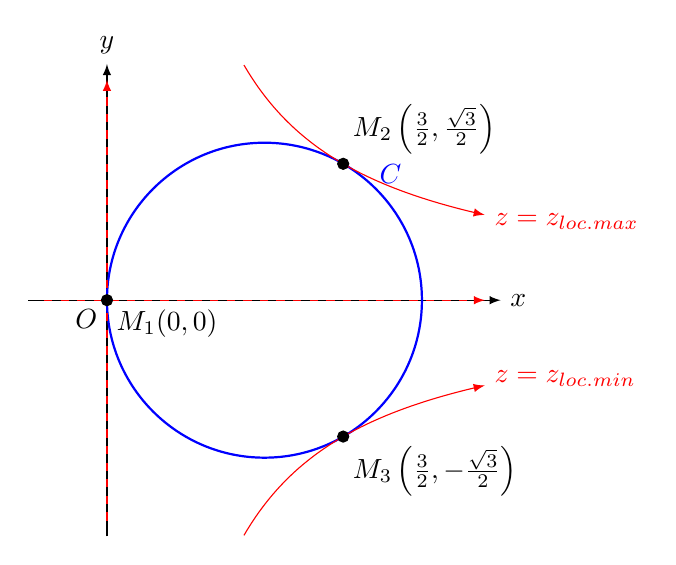
\begin{tikzpicture}[-latex, scale=2]
            % 坐标轴
            \draw ( -0.5, 0) -- (2.5, 0) node[right] {$x$};
            \draw (0, -1.5) -- (0, 1.5) node[above] {$y$};
            \node[below left] at (0,0) {$O$};

            % 约束圆
            \draw[thick, blue] (1, 0) circle (1);
            \node[blue] at (1.8, 0.8) {$C$};

            % 等值线 xy = 0 (坐标轴)
            \draw[dashed, red] (0, -1.4) -- (0, 1.4);
            \draw[dashed, red] (-0.4, 0) -- (2.4, 0);

            % 等值线 xy = 3*sqrt(3)/4 (约 1.299)
            \draw[samples=100, domain=0.87:2.4, smooth, red] plot (\x, {1.299/\x});
            \node[red, right] at (2.4, 0.5) {$z = z_{\text{loc.max}}$};

            % 等值线 xy = -3*sqrt(3)/4 (约 -1.299)
            \draw[samples=100, domain=0.87:2.4, smooth, red] plot (\x, {-1.299/\x});
            \node[red, right] at (2.4, -0.5) {$z = z_{\text{loc.min}}$};

            % 极值点标注
            \filldraw (0,0) circle (1pt) node[below right] {$M_1(0,0)$};
            \filldraw (1.5, 0.866) circle (1pt) node[above right] {$M_2\left(\frac{3}{2}, \frac{\sqrt{3}}{2}\right)$};
            \filldraw (1.5, -0.866) circle (1pt) node[below right] {$M_3\left(\frac{3}{2}, -\frac{\sqrt{3}}{2}\right)$};
        \end{tikzpicture}
    \end{center}

    根据拉格朗日乘数法，极值点分别为：
    \begin{equation}
        \begin{aligned}
            M_1 & = (0, 0),                                          \\
            M_2 & = \left( \frac{3}{2}, \frac{\sqrt{3}}{2} \right),  \\
            M_3 & = \left( \frac{3}{2}, -\frac{\sqrt{3}}{2} \right).
        \end{aligned}
    \end{equation}

    其中 $M_1$ 为等值线 $z=0$ 与圆的交点（非切点），而 $M_2$ 与 $M_3$ 为等值线与圆的切点，分别对应最大值与最小值。

    \begin{equation}
        \boxed{z_{\text{loc.max}} = \frac{3\sqrt{3}}{4}, \quad z_{\text{loc.min}} = -\frac{3\sqrt{3}}{4}}
    \end{equation}
\end{solution}


\begin{problem}{条件极值}{Constrained-Extrema}
    求下列函数在指定条件下的极值
    \begin{enumerate}
        \item $u = x^{2} + y^{2}$, 若 $\frac{x}{a} + \frac{y}{b} = 1$;
        \item $u = x + y + z$, 若 $\frac{1}{x} + \frac{1}{y} + \frac{1}{z} = 1, x > 0, y > 0, z > 0$;
        \item $u = \sin x \sin y \sin z$, 若 $x + y + z = \frac{\uppi}{2}, x > 0, y > 0, z > 0$;
        \item $u = x y z$, 若 $x + y + z = 0$ 且 $x^{2} + y^{2} + z^{2} = 1$.
    \end{enumerate}
\end{problem}

\begin{solution}
    \ansitem{1}

    构造拉格朗日函数 $L(x, y, \lambda) = x^{2} + y^{2} + \lambda \left( \frac{x}{a} + \frac{y}{b} - 1 \right)$。令其偏导数为零：
    \begin{equation}
        \label{eq:p1-lagrange}
        \begin{cases}
            2x + \frac{\lambda}{a} = 0, \\
            2y + \frac{\lambda}{b} = 0, \\
            \frac{x}{a} + \frac{y}{b} = 1.
        \end{cases}
    \end{equation}
    由前两式得 $x = -\frac{\lambda}{2a}, y = -\frac{\lambda}{2b}$，代入约束条件可得：
    \begin{equation}
        -\frac{\lambda}{2 a^{2}} - \frac{\lambda}{2 b^{2}} = 1 \implies \lambda = -\frac{2 a^{2} b^{2}}{a^{2} + b^{2}}.
    \end{equation}
    此时 $x = \frac{a b^{2}}{a^{2} + b^{2}}, y = \frac{a^{2} b}{a^{2} + b^{2}}$，代入 $u$ 的表达式计算极小值：
    \begin{equation}
        \boxed{u = \frac{a^{2} b^{2}}{a^{2} + b^{2}}}.
    \end{equation}

    \ansitem{2}

    构造拉格朗日函数 $L(x, y, z, \lambda) = x + y + z + \lambda \left( \frac{1}{x} + \frac{1}{y} + \frac{1}{z} - 1 \right)$。求偏导数：
    \begin{equation}
        \begin{cases}
            1 - \frac{\lambda}{x^{2}} = 0, \\
            1 - \frac{\lambda}{y^{2}} = 0, \\
            1 - \frac{\lambda}{z^{2}} = 0.
        \end{cases}
    \end{equation}
    结合 $x, y, z > 0$，可得 $x = y = z = \sqrt{\lambda}$。代入约束条件：
    \begin{equation}
        \frac{3}{\sqrt{\lambda}} = 1 \implies \sqrt{\lambda} = 3 \implies x = y = z = 3.
    \end{equation}
    代入 $u$ 得到极小值：
    \begin{equation}
        \boxed{u = 9}.
    \end{equation}

    \ansitem{3}

    构造拉格朗日函数 $L(x, y, z, \lambda) = \sin x \sin y \sin z + \lambda \left( x + y + z - \frac{\uppi}{2} \right)$。令偏导数为零：
    \begin{equation}
        \begin{cases}
            \cos x \sin y \sin z + \lambda = 0, \\
            \sin x \cos y \sin z + \lambda = 0, \\
            \sin x \sin y \cos z + \lambda = 0.
        \end{cases}
    \end{equation}
    由上式可得 $\cos x \sin y \sin z = \sin x \cos y \sin z = \sin x \sin y \cos z$。由于 $x, y, z \in (0, \uppi/2)$，上式等价于：
    \begin{equation}
        \cot x = \cot y = \cot z \implies x = y = z.
    \end{equation}
    由约束条件 $3x = \frac{\uppi}{2}$ 得 $x = y = z = \frac{\uppi}{6}$，极高值为：
    \begin{equation}
        \boxed{u = \frac{1}{8}}.
    \end{equation}

    \ansitem{4}

    构造拉格朗日函数 $L(x, y, z, \lambda_1, \lambda_2) = x y z + \lambda_{1}(x + y + z) + \lambda_{2}(x^{2} + y^{2} + z^{2} - 1)$。求偏导数：
    \begin{equation}
        \begin{cases}
            y z + \lambda_{1} + 2 \lambda_{2} x = 0, \\
            x z + \lambda_{1} + 2 \lambda_{2} y = 0, \\
            x y + \lambda_{1} + 2 \lambda_{2} z = 0.
        \end{cases}
    \end{equation}
    相邻两式相减可得 $(y - x)(z - 2 \lambda_{2}) = 0$, $(z - y)(x - 2 \lambda_{2}) = 0$, $(x - z)(y - 2 \lambda_{2}) = 0$。若 $x, y, z$ 互不相等，则必有 $x = y = z = 2 \lambda_{2}$，产生矛盾。故至少有两项相等。设 $x = y$，由 $x + y + z = 0$ 得 $z = -2x$。代入 $x^{2} + y^{2} + z^{2} = 1$：
    \begin{equation}
        x^{2} + x^{2} + 4x^{2} = 1 \implies 6x^{2} = 1 \implies x = \pm \frac{1}{\sqrt{6}}.
    \end{equation}
    当 $x = y = \frac{1}{\sqrt{6}}, z = -\frac{2}{\sqrt{6}}$ 时，$u = -\frac{\sqrt{6}}{18}$；当 $x = y = -\frac{1}{\sqrt{6}}, z = \frac{2}{\sqrt{6}}$ 时，$u = \frac{\sqrt{6}}{18}$。由对称性，函数在指定条件下极值为：
    \begin{equation}
        \boxed{u = \pm \frac{\sqrt{6}}{18}}.
    \end{equation}
\end{solution}


\begin{problem}{多元函数最值}{Extremum-of-Multivariate-Functions}
    求下列函数在指定范围内的最大值与最小值.
    \begin{enumerate}
        \item $z = x^2 - y^2$, $\{(x, y) \mid x^2 + y^2 \le 4\}$;
        \item $z = x^2 - xy + y^2$, $\{(x, y) \mid |x| + |y| \le 1\}$;
        \item $z = \sin x + \sin y - \sin(x + y)$, $\{(x, y) \mid x \ge 0, y \ge 0, x + y \le 2 \uppi\}$;
        \item $z = x^2 y(4 - x - y)$, $\{(x, y) \mid x \ge 0, y \ge 0, x + y \le 6\}$.
    \end{enumerate}
\end{problem}

\begin{solution}
    \ansitem{1}
    考察区域内部的极值点，由 $\frac{\partial z}{\partial x} = 2x = 0$，$\frac{\partial z}{\partial y} = -2y = 0$ 得驻点 $(0, 0)$，此时 $z(0, 0) = 0$。

    在边界 $x^2 + y^2 = 4$ 上，有 $y^2 = 4 - x^2$，代入原式得
    \begin{equation}
        z = x^2 - (4 - x^2) = 2x^2 - 4, \quad x \in [-2, 2].
    \end{equation}
    当 $x = \pm 2$ 时，$z = 4$；当 $x = 0$ 时，$z = -4$。
    \begin{equation}
        \boxed{z_{\max} = 4, \quad z_{\min} = -4}
    \end{equation}

    \ansitem{2}
    考察内部，由 $\frac{\partial z}{\partial x} = 2x - y = 0$ 与 $\frac{\partial z}{\partial y} = 2y - x = 0$ 得驻点 $(0, 0)$，此时 $z(0, 0) = 0$。

    边界为由 $(1, 0), (0, 1), (-1, 0), (0, -1)$ 围成的正方形。
    在第一象限边界 $x + y = 1$（$x \in [0, 1]$）上：
    \begin{equation}
        z = x^2 - x(1 - x) + (1 - x)^2 = 3x^2 - 3x + 1.
    \end{equation}
    其在 $x = \frac{1}{2}$ 处取得局部最小 $z = \frac{1}{4}$，在端点处 $z = 1$。
    在第四象限边界 $x - y = 1$（$x \in [0, 1]$）上：
    \begin{equation}
        z = x^2 - x(x - 1) + (x - 1)^2 = x^2 - x + 1.
    \end{equation}
    其在 $x = \frac{1}{2}$ 处取得局部最小 $z = \frac{3}{4}$，在端点处 $z = 1$。
    由对称性可知，边界上的最大值为 $1$，最小值为 $\frac{1}{4}$。
    \begin{equation}
        \boxed{z_{\max} = 1, \quad z_{\min} = 0}
    \end{equation}

    \ansitem{3}
    利用积化和差公式，原函数可化为
    \begin{equation}
        z = 4 \sin \frac{x}{2} \sin \frac{y}{2} \sin \frac{x + y}{2}.
    \end{equation}
    在给定区域 $x \ge 0, y \ge 0, x + y \le 2\uppi$ 内，由于 $\frac{x}{2}, \frac{y}{2}, \frac{x + y}{2} \in [0, \uppi]$，故 $z \ge 0$。
    边界 $x = 0, y = 0, x + y = 2\uppi$ 上 $z$ 均为 $0$，故最小值 $z_{\min} = 0$。

    考察内部驻点：
    \begin{equation}
        \begin{aligned}
            \frac{\partial z}{\partial x} & = \cos x - \cos(x + y) = 0 \implies \cos x = \cos(x + y), \\
            \frac{\partial z}{\partial y} & = \cos y - \cos(x + y) = 0 \implies \cos y = \cos(x + y).
        \end{aligned}
    \end{equation}
    由 $\cos x = \cos y$ 且 $0 < x, y < 2\uppi$，$x + y < 2\uppi$ 得 $x = y$。
    代入得 $\cos x = \cos 2x$，解得 $x = \frac{2\uppi}{3}$。此时 $z = \sin \frac{2\uppi}{3} + \sin \frac{2\uppi}{3} - \sin \frac{4\uppi}{3} = \frac{3\sqrt{3}}{2}$。
    \begin{equation}
        \boxed{z_{\max} = \frac{3\sqrt{3}}{2}, \quad z_{\min} = 0}
    \end{equation}

    \ansitem{4}
    在边界 $x = 0, y = 0$ 上 $z = 0$。在边界 $x + y = 6$ 上，$z = x^2(6 - x)(-2) = 2x^3 - 12x^2$。
    设 $f(x) = 2x^3 - 12x^2$（$x \in [0, 6]$），则 $f'(x) = 6x(x - 4)$。当 $x = 4$ 时，取得极小值 $f(4) = -64$。

    考察内部驻点：
    \begin{equation}
        \begin{aligned}
            \frac{\partial z}{\partial x} & = 2xy(4 - x - y) - x^2 y = xy(8 - 3x - 2y) = 0, \\
            \frac{\partial z}{\partial y} & = x^2(4 - x - y) - x^2 y = x^2(4 - x - 2y) = 0.
        \end{aligned}
    \end{equation}
    在 $x > 0, y > 0$ 时，联立 $3x + 2y = 8$ 与 $x + 2y = 4$，解得 $x = 2, y = 1$。
    此时 $z(2, 1) = 2^2 \cdot 1 \cdot (4 - 2 - 1) = 4$。比较上述各点：
    \begin{equation}
        \boxed{z_{\max} = 4, \quad z_{\min} = -64}
    \end{equation}
\end{solution}


\begin{problem}{距离平方和最小}{Distance-Square-Sum}
    在平面 $3x - 2z = 0$ 上求一点，使它与点 $A(1, 1, 1)$ 和 $B(2, 3, 4)$ 的距离平方和最小。
\end{problem}

\begin{solution}
    设所求点为 $P(x, y, z)$，目标函数为 $P$ 到 $A, B$ 两点距离的平方和：
    \begin{equation}
        f(x, y, z) = (x-1)^2 + (y-1)^2 + (z-1)^2 + (x-2)^2 + (y-3)^2 + (z-4)^2
    \end{equation}
    约束条件为 $g(x, y, z) = 3x - 2z = 0$。构造 Lagrange 函数：
    \begin{equation}
        L(x, y, z, \lambda) = (x-1)^2 + (y-1)^2 + (z-1)^2 + (x-2)^2 + (y-3)^2 + (z-4)^2 + \lambda(3x - 2z)
    \end{equation}
    对其求偏导数并令其为零：
    \begin{equation}
        \begin{cases}
            L_x = 2(x-1) + 2(x-2) + 3\lambda = 4x - 6 + 3\lambda = 0  \\
            L_y = 2(y-1) + 2(y-3) = 4y - 8 = 0                        \\
            L_z = 2(z-1) + 2(z-4) - 2\lambda = 4z - 10 - 2\lambda = 0 \\
            3x - 2z = 0
        \end{cases}
    \end{equation}
    由第二式得 $y = 2$。由第一、三式消去 $\lambda$ 得：
    \begin{equation}
        2(4x - 6) + 3(4z - 10) = 0 \implies 8x + 12z = 42 \implies 4x + 6z = 21
    \end{equation}
    代入 $z = \frac{3}{2}x$ 可得：
    \begin{equation}
        4x + 6\left( \frac{3}{2}x \right) = 13x = 21 \implies x = \frac{21}{13}
    \end{equation}
    进而解得 $z = \frac{63}{26}$。故所求点为：
    \begin{equation}
        \boxed{P = \left( \frac{21}{13}, 2, \frac{63}{26} \right)}
    \end{equation}
\end{solution}

\begin{problem}{空间曲线极值}{Curve-Extremum}
    在曲线 $\begin{cases} z = x^2 + 2y^2 \\ z = 6 - 2x^2 - y^2 \end{cases}$ 上，求竖坐标分别为最大值和最小值的点。
\end{problem}

\begin{solution}
    消去 $z$ 可得曲线在 $Oxy$ 平面上的投影曲线方程：
    \begin{equation}
        x^2 + 2y^2 = 6 - 2x^2 - y^2 \implies 3x^2 + 3y^2 = 6 \implies x^2 + y^2 = 2
    \end{equation}
    在曲线上，竖坐标 $z$ 可表示为：
    \begin{equation}
        z = x^2 + 2y^2 = (x^2 + y^2) + y^2 = 2 + y^2
    \end{equation}
    由 $x^2 + y^2 = 2$ 可知 $0 \le y^2 \le 2$。
    当 $y^2 = 0$ 即 $y = 0$ 时，$z$ 取得最小值 $z_{\min} = 2$，此时 $x = \pm\sqrt{2}$。
    当 $y^2 = 2$ 即 $y = \pm\sqrt{2}$ 时，$z$ 取得最大值 $z_{\max} = 4$，此时 $x = 0$。
    综上所述，竖坐标最小的点为 $(\pm\sqrt{2}, 0, 2)$，竖坐标最大的点为 $(0, \pm\sqrt{2}, 4)$。
    \begin{equation}
        \boxed{P_{\max} = (0, \pm\sqrt{2}, 4), \quad P_{\min} = (\pm\sqrt{2}, 0, 2)}
    \end{equation}
\end{solution}

\begin{problem}{极值点判定}{Extremum-Point-Verification}
    设 $f(x, y) = 3x^2y - x^4 - 2y^2$。证明：$(0, 0)$ 不是它的极值点，但沿过 $(0, 0)$ 点的每条直线，$(0, 0)$ 都是它的极大值点。
\end{problem}

\begin{myproof}
    首先，将原函数分解因式：
    \begin{equation}
        f(x, y) = -(x^4 - 3x^2y + 2y^2) = -(x^2 - y)(x^2 - 2y)
    \end{equation}
    显然 $f(0, 0) = 0$。在 $(0, 0)$ 的任意邻域内：
    若取点满足 $y = \frac{3}{4}x^2$，则 $f(x, \frac{3}{4}x^2) = -(x^2 - \frac{3}{4}x^2)(x^2 - \frac{3}{2}x^2) = \frac{1}{8}x^4 > 0$；
    若取点满足 $y = 0$，则 $f(x, 0) = -x^4 < 0$。
    由于在 $(0, 0)$ 的任意邻域内 $f(x, y)$ 均可取正值和负值，故 $(0, 0)$ 不是极值点。

    其次，考虑过原点的任意直线 $L$。若直线为 $x = 0$，则 $f(0, y) = -2y^2$，在 $y = 0$ 处取得极大值。
    若直线为 $y = kx$，令 $g(x) = f(x, kx)$：
    \begin{equation}
        g(x) = 3kx^3 - x^4 - 2k^2x^2 = x^2(3kx - x^2 - 2k^2)
    \end{equation}
    当 $k \neq 0$ 时，有：
    \begin{equation}
        g'(x) = 9kx^2 - 4x^3 - 4k^2x, \quad g'(0) = 0
    \end{equation}
    \begin{equation}
        g''(x) = 18kx - 12x^2 - 4k^2, \quad g''(0) = -4k^2 < 0
    \end{equation}
    根据二阶导数判别法，$x = 0$ 是 $g(x)$ 的极大值点。
    若 $k = 0$，则 $g(x) = -x^4$，显然在 $x = 0$ 处取得极大值。
    综上，沿过 $(0, 0)$ 的每条直线，$(0, 0)$ 均为极大值点。
\end{myproof}


\begin{problem}{条件极值}{Tent-Surface-Area}
    一帐篷, 下部为圆柱形, 上部盖以圆锥形的顶篷, 设帐篷的容积为一定数 $V_0$。
    试证当 $R = \sqrt{5}H, h = 2H$ 时, (其中 $R, H$ 各为圆柱形的底半径和高, $h$ 为圆锥形的高)，所用蓬布最省。
\end{problem}

\begin{myproof}
    设帐篷的表面积为 $S$, 由题意可知, 容积约束为
    \begin{equation}\label{eq:volume-const-1}
        V = \uppi R^2 H + \frac{1}{3} \uppi R^2 h = V_0 .
    \end{equation}
    所用蓬布面积（侧面积之和）为
    \begin{equation}\label{eq:surface-area-1}
        S(R, H, h) = 2 \uppi R H + \uppi R \sqrt{R^2 + h^2} .
    \end{equation}
    构造拉格朗日函数
    \begin{equation}
        L(R, H, h, \lambda) = 2 \uppi R H + \uppi R \sqrt{R^2 + h^2} + \lambda \left( \uppi R^2 H + \frac{1}{3} \uppi R^2 h - V_0 \right) .
    \end{equation}
    对各变量求偏导并令其为零
    \begin{equation}\label{eq:partial-H}
        \frac{\partial L}{\partial H} = 2 \uppi R + \lambda \uppi R^2 = 0 \implies \lambda = -\frac{2}{R} ,
    \end{equation}
    \begin{equation}\label{eq:partial-h}
        \frac{\partial L}{\partial h} = \frac{\uppi R h}{\sqrt{R^2 + h^2}} + \frac{1}{3} \lambda \uppi R^2 = 0 .
    \end{equation}
    将 $\lambda = -2/R$ 代入 \zcref{eq:partial-h} 得
    \begin{equation}
        \frac{h}{\sqrt{R^2 + h^2}} = \frac{2}{3} \implies 9h^2 = 4(R^2 + h^2) \implies R = \frac{\sqrt{5}}{2}h .
    \end{equation}
    再对 $R$ 求偏导
    \begin{equation}
        \frac{\partial L}{\partial R} = 2 \uppi H + \uppi \sqrt{R^2 + h^2} + \frac{\uppi R^2}{\sqrt{R^2 + h^2}} + \lambda \left( 2 \uppi R H + \frac{2}{3} \uppi R h \right) = 0 .
    \end{equation}
    代入 $\lambda = -2/R$ 并化简
    \begin{equation}
        \begin{aligned}
                     & 2 \uppi H + \frac{\uppi (2R^2 + h^2)}{\sqrt{R^2 + h^2}} - \frac{2}{R} \left( 2 \uppi R H + \frac{2}{3} \uppi R h \right) = 0 \\
            \implies & -2 \uppi H + \frac{\uppi (2R^2 + h^2)}{\sqrt{R^2 + h^2}} - \frac{4}{3} \uppi h = 0 .
        \end{aligned}
    \end{equation}
    利用 $R^2 = \frac{5}{4}h^2$ 及 $\sqrt{R^2 + h^2} = \frac{3}{2}h$ 代入上式
    \begin{equation}
        \begin{aligned}
                     & \frac{\uppi \left( 2 \cdot \frac{5}{4}h^2 + h^2 \right)}{\frac{3}{2}h} = 2 \uppi H + \frac{4}{3} \uppi h \\
            \implies & \frac{7}{3} \uppi h = 2 \uppi H + \frac{4}{3} \uppi h \implies \uppi h = 2 \uppi H \implies h = 2H .
        \end{aligned}
    \end{equation}
    此时 $R = \frac{\sqrt{5}}{2}(2H) = \sqrt{5}H$. 故结论成立.
\end{myproof}

\begin{problem}{均值不等式}{Parallelepiped-Max-Volume}
    已知平行六面体所有各棱长之和为 $12a$, 求其最大体积。
\end{problem}

\begin{solution}
    设平行六面体的三组棱长分别为 $x, y, z$. 显然当其为长方体时体积最大.
    由题意得约束条件
    \begin{equation}
        4(x + y + z) = 12a \implies x + y + z = 3a .
    \end{equation}
    其体积为 $V = xyz$. 根据算术-几何平均值不等式
    \begin{equation}
        V = xyz \le \left( \frac{x + y + z}{3} \right)^3 = \left( \frac{3a}{3} \right)^3 = a^3 .
    \end{equation}
    等号成立当且仅当 $x = y = z = a$, 即该平行六面体为棱长为 $a$ 的正方体.
    \begin{equation}
        \boxed{V_{\max} = a^3}
    \end{equation}
\end{solution}

\begin{problem}{切线方程与极值}{Ellipse-Tangent-Triangle}
    在椭圆 $\frac{x^2}{a^2} + \frac{y^2}{b^2} = 1$ 上求一点 $M(x, y) (x, y \ge 0)$, 使椭圆在该点的切线与坐标轴构成的三角形面积为最小, 并求其面积。
\end{problem}

\begin{solution}
    \ansitem{1}
    设椭圆上一点为 $M(x_0, y_0)$, 则该点处的切线方程为
    \begin{equation}
        \frac{x_0 x}{a^2} + \frac{y_0 y}{b^2} = 1 .
    \end{equation}
    该切线在坐标轴上的截距分别为 $X = \frac{a^2}{x_0}$ 和 $Y = \frac{b^2}{y_0}$. 围成的三角形面积为
    \begin{equation}
        S = \frac{1}{2} XY = \frac{a^2 b^2}{2 x_0 y_0} .
    \end{equation}
    由于 $\frac{x_0^2}{a^2} + \frac{y_0^2}{b^2} = 1$, 由均值不等式得
    \begin{equation}
        1 = \frac{x_0^2}{a^2} + \frac{y_0^2}{b^2} \ge 2 \sqrt{\frac{x_0^2 y_0^2}{a^2 b^2}} = \frac{2 x_0 y_0}{ab} \implies x_0 y_0 \le \frac{ab}{2} .
    \end{equation}
    当且仅当 $\frac{x_0^2}{a^2} = \frac{y_0^2}{b^2} = \frac{1}{2}$, 即 $x_0 = \frac{a}{\sqrt{2}}, y_0 = \frac{b}{\sqrt{2}}$ 时面积最小.
    \begin{equation}
        \boxed{M = \left( \frac{a}{\sqrt{2}}, \frac{b}{\sqrt{2}} \right)}
    \end{equation}

    \ansitem{2}
    将极值点坐标代入面积公式得
    \begin{equation}
        S_{\min} = \frac{a^2 b^2}{2 \cdot \frac{a}{\sqrt{2}} \cdot \frac{b}{\sqrt{2}}} = ab .
    \end{equation}
    \begin{equation}
        \boxed{S_{\min} = ab}
    \end{equation}
\end{solution}


\begin{problem}{距离平方和最小值}{sum-of-squared-distances}
    求平面上一点 $(x_0, y_0)$，使其到 $n$ 个定点 $(x_1, y_1), (x_2, y_2), \dots, (x_n, y_n)$ 的距离的平方和最小。
\end{problem}

\begin{solution}
    设目标函数为 $f(x_0, y_0)$，表示该点到各定点距离的平方和：
    \begin{equation}
        f(x_0, y_0) = \sum_{i=1}^{n} \left[ (x_0 - x_i)^2 + (y_0 - y_i)^2 \right].
    \end{equation}
    为了求其极小值点，分别对 $x_0$ 和 $y_0$ 求偏导数并令其为 $0$：
    \begin{equation}
        \begin{aligned}
            \frac{\partial f}{\partial x_0} & = \sum_{i=1}^{n} 2(x_0 - x_i) = 2nx_0 - 2\sum_{i=1}^{n} x_i = 0, \\
            \frac{\partial f}{\partial y_0} & = \sum_{i=1}^{n} 2(y_0 - y_i) = 2ny_0 - 2\sum_{i=1}^{n} y_i = 0.
        \end{aligned}
    \end{equation}
    解得驻点坐标为：
    \begin{equation}
        x_0 = \frac{1}{n} \sum_{i=1}^{n} x_i, \quad y_0 = \frac{1}{n} \sum_{i=1}^{n} y_i.
    \end{equation}
    由于 $f(x_0, y_0)$ 是关于 $x_0, y_0$ 的开口向上的二次曲面，该驻点即为全局最小值点，对应几何上的形心。
    \begin{equation}
        \boxed{(x_0, y_0) = \left( \frac{1}{n} \sum_{i=1}^{n} x_i, \frac{1}{n} \sum_{i=1}^{n} y_i \right)}
    \end{equation}
\end{solution}


\begin{problem}{椭球内接长方体最大体积}{max-volume-ellipsoid-box}
    椭球体 $\frac{x^2}{a^2} + \frac{y^2}{b^2} + \frac{z^2}{c^2} \le 1$ 的内接长方体中，求体积最大的长方体的体积。
\end{problem}

\begin{solution}
    设长方体在第一卦限内的顶点为 $(x, y, z)$，其中 $x, y, z > 0$。根据对称性，长方体的体积 $V$ 为：
    \begin{equation}
        V = (2x)(2y)(2z) = 8xyz.
    \end{equation}
    该顶点位于椭球面上，满足约束条件：
    \begin{equation}
        \frac{x^2}{a^2} + \frac{y^2}{b^2} + \frac{z^2}{c^2} = 1.
    \end{equation}
    利用算术-几何平均值不等式（AM-GM Inequality）：
    \begin{equation}
        \frac{\frac{x^2}{a^2} + \frac{y^2}{b^2} + \frac{z^2}{c^2}}{3} \ge \sqrt[3]{\frac{x^2 y^2 z^2}{a^2 b^2 c^2}}.
    \end{equation}
    将约束条件代入上式，得：
    \begin{equation}
        \frac{1}{3} \ge \left( \frac{xyz}{abc} \right)^{\frac{2}{3}} \implies xyz \le \frac{abc}{3\sqrt{3}}.
    \end{equation}
    当且仅当 $\frac{x^2}{a^2} = \frac{y^2}{b^2} = \frac{z^2}{c^2} = \frac{1}{3}$ 时等号成立。此时体积取得最大值：
    \begin{equation}
        V_{\max} = 8 \cdot \frac{abc}{3\sqrt{3}} = \frac{8\sqrt{3} abc}{9}.
    \end{equation}
    \begin{equation}
        \boxed{V_{\max} = \frac{8\sqrt{3} abc}{9}}
    \end{equation}
\end{solution}


\begin{problem}{旋转椭球面到平面的最值点}{distance-ellipsoid-plane}
    在旋转椭球面 $\frac{x^2}{4} + y^2 + z^2 = 1$ 上求距平面 $x + y + 2z = 9$ 最远和最近的点。
\end{problem}

\begin{solution}
    椭球面上一点 $(x, y, z)$ 到平面 $x + y + 2z - 9 = 0$ 的距离 $d$ 为：
    \begin{equation}
        d = \frac{|x + y + 2z - 9|}{\sqrt{1^2 + 1^2 + 2^2}} = \frac{|x + y + 2z - 9|}{\sqrt{6}}.
    \end{equation}
    令 $u = x + y + 2z$。构造 Lagrange 函数以求 $u$ 在 $\frac{x^2}{4} + y^2 + z^2 = 1$ 下的最值：
    \begin{equation}
        F(x, y, z, \lambda) = x + y + 2z + \lambda \left( \frac{x^2}{4} + y^2 + z^2 - 1 \right).
    \end{equation}
    令偏导数为 $0$：
    \begin{equation}
        F_x = 1 + \frac{\lambda x}{2} = 0, \quad F_y = 1 + 2\lambda y = 0, \quad F_z = 2 + 2\lambda z = 0.
    \end{equation}
    得到 $x = -\frac{2}{\lambda}, y = -\frac{1}{2\lambda}, z = -\frac{1}{\lambda}$，代入椭球面方程：
    \begin{equation}
        \frac{1}{4} \left( -\frac{2}{\lambda} \right)^2 + \left( -\frac{1}{2\lambda} \right)^2 + \left( -\frac{1}{\lambda} \right)^2 = \frac{9}{4\lambda^2} = 1 \implies \lambda = \pm \frac{3}{2}.
    \end{equation}

    \ansitem{1} 最近点：

    当 $\lambda = -\frac{3}{2}$ 时，对应坐标为 $\left( \frac{4}{3}, \frac{1}{3}, \frac{2}{3} \right)$。此时 $u = 3$，距离 $d = \frac{|3-9|}{\sqrt{6}} = \sqrt{6}$。

    \ansitem{2} 最远点：

    当 $\lambda = \frac{3}{2}$ 时，对应坐标为 $\left( -\frac{4}{3}, -\frac{1}{3}, -\frac{2}{3} \right)$。此时 $u = -3$，距离 $d = \frac{|-3-9|}{\sqrt{6}} = 2\sqrt{6}$。

    \begin{equation}
        \boxed{\text{最近点为} \left( \frac{4}{3}, \frac{1}{3}, \frac{2}{3} \right), \text{最远点为} \left( -\frac{4}{3}, -\frac{1}{3}, -\frac{2}{3} \right)}
    \end{equation}
\end{solution}


\begin{problem}{曲面切平面与体积最值}{Surface-Tangent-Volume}
    设曲面 $S: \sqrt{x} + \sqrt{y} + \sqrt{z} = \sqrt{a} \, (a > 0)$。
    \begin{enumerate}
        \item 证明 $S$ 上任意点处的切平面与各坐标轴的截距之和等于 $a$。
        \item 在 $S$ 上求一切平面，使此切平面与三坐标面所围成的四面体体积最大，并求四面体体积的最大值。
    \end{enumerate}
\end{problem}

\begin{solution}
    \ansitem{1}

    设 $P_0(x_0, y_0, z_0)$ 为曲面 $S$ 上任一点，令 $F(x, y, z) = \sqrt{x} + \sqrt{y} + \sqrt{z} - \sqrt{a}$。计算该点处的梯度向量：
    \begin{equation}
        \nabla F\big|_{P_0} = \left( \frac{1}{2\sqrt{x_0}}, \frac{1}{2\sqrt{y_0}}, \frac{1}{2\sqrt{z_0}} \right).
    \end{equation}
    则 $P_0$ 处的切平面方程为
    \begin{equation}
        \frac{1}{2\sqrt{x_0}}(x - x_0) + \frac{1}{2\sqrt{y_0}}(y - y_0) + \frac{1}{2\sqrt{z_0}}(z - z_0) = 0.
    \end{equation}
    整理可得
    \begin{equation}
        \frac{x}{\sqrt{x_0}} + \frac{y}{\sqrt{y_0}} + \frac{z}{\sqrt{z_0}} = \sqrt{x_0} + \sqrt{y_0} + \sqrt{z_0}.
    \end{equation}
    由于 $P_0$ 在曲面 $S$ 上，满足 $\sqrt{x_0} + \sqrt{y_0} + \sqrt{z_0} = \sqrt{a}$，代入上式并化为截距式：
    \begin{equation}
        \frac{x}{\sqrt{ax_0}} + \frac{y}{\sqrt{ay_0}} + \frac{z}{\sqrt{az_0}} = 1.
    \end{equation}
    因此，切平面在各坐标轴上的截距分别为 $X = \sqrt{ax_0}$、$Y = \sqrt{ay_0}$、$Z = \sqrt{az_0}$。其截距之和为
    \begin{equation}
        X + Y + Z = \sqrt{a}(\sqrt{x_0} + \sqrt{y_0} + \sqrt{z_0}) = \sqrt{a} \cdot \sqrt{a} = a.
    \end{equation}
    结论成立。

    \ansitem{2}

    由第 (1) 问可知，四面体的体积 $V$ 为
    \begin{equation}
        V = \frac{1}{6} XYZ = \frac{1}{6} a\sqrt{a} \sqrt{x_0 y_0 z_0}.
    \end{equation}
    根据算术—几何平均值不等式，在 $\sqrt{x_0} + \sqrt{y_0} + \sqrt{z_0} = \sqrt{a}$ 的约束下：
    \begin{equation}
        \sqrt[3]{\sqrt{x_0 y_0 z_0}} \le \frac{\sqrt{x_0} + \sqrt{y_0} + \sqrt{z_0}}{3} = \frac{\sqrt{a}}{3}.
    \end{equation}
    两边同时立方可得
    \begin{equation}
        \sqrt{x_0 y_0 z_0} \le \left( \frac{\sqrt{a}}{3} \right)^3 = \frac{a\sqrt{a}}{27}.
    \end{equation}
    当且仅当 $\sqrt{x_0} = \sqrt{y_0} = \sqrt{z_0} = \frac{\sqrt{a}}{3}$，即 $x_0 = y_0 = z_0 = \frac{a}{9}$ 时，等号成立。此时切平面方程为
    \begin{equation}
        \frac{x}{\sqrt{a \cdot \frac{a}{9}}} + \frac{y}{\sqrt{a \cdot \frac{a}{9}}} + \frac{z}{\sqrt{a \cdot \frac{a}{9}}} = 1 \implies x + y + z = \frac{a}{3}.
    \end{equation}
    体积的最大值为
    \begin{equation}
        V_{\max} = \frac{1}{6} a\sqrt{a} \cdot \frac{a\sqrt{a}}{27} = \frac{a^3}{162}.
    \end{equation}
    综上所述，最大体积及其对应的切平面方程为
    \begin{equation}
        \boxed{x + y + z = \frac{a}{3}, \quad V_{\max} = \frac{a^3}{162}}
    \end{equation}
\end{solution}

\endinput
